\section{Statistical Analysis of Mock Dataset}

There are \(5\) plain text files given, called \(v_1\), \(v_2\), \(v_3\), \(v_4\) and \(v_5\).
(\(v_1\) is short for variable \(1\), \etc{}) Each text file contains \(1600000\) lines,
which correspond to
measurements of the given variable from a simulation. There are autocorrelations
(correlations in time or measurement number) for each variable. There are also correlations
between variables. In this problem, you need to analyze this data, using the methods
discussed in class, to find average values, standard deviations of means, autocorrelations,
etc.

We will use \(M\) to represent the total number of values, i.e. \(M = 1600000\). \(M\) is large
enough so that it represents an effectively ``infinite'' sample size. Thus, the true data
mean can be well approximated by averaging over all \(M\) values. Averages, standard
deviations, \etc, determined from the ``infinite'' sample will be denoted with a hat, i.e.
\(\barhat{v}_1\), \etc.

We will use \(N\) to represent the number of measurements in a sample of the data. \(N\)
corresponds to the amount of data you might actually collect in a simulation.


\Question{} Determine the true means, \(\barhat{v}_a\) for \(v_1\), \(v_2\), \(\ldots\),
\(v_5\) from all \(M\) values.

\Answer{}
First, we need to define two types: the population (universe of the data) and the samples,
as shown in Snippet~\ref{lst:types}.

\begin{algorithm}
    \caption{The \code{Population} type and the \code{Sample} type.}
    \label{lst:types}
    \begin{juliacode}
        struct Population{T} <: AbstractVector{T}
            data::Vector{T}
        end

        struct Sample{T} <: AbstractVector{T}
            data::Vector{T}
        end
    \end{juliacode}
\end{algorithm}

Now, we need to read the data from each file. This is pretty simple since all \(5\) files
are plain text files. The method is shown in function \code{read} in
Snippet~\ref{lst:readdata}.

\begin{algorithm}
    \caption{Function \code{read} is used to read data from each file.}
    \label{lst:readdata}
    \begin{juliacode}
        function Base.read(filename::AbstractString, ::Type{Population})
            open(filename, "r") do io
                read(io, Population)
            end
        end
        function Base.read(io::IO, ::Type{Population})
            return Population(
                map(eachline(io)) do line
                    parse(Float64, strip(line))
                end,
            )
        end
    \end{juliacode}
\end{algorithm}

The definition of the true mean is
\begin{equation}
    \barhat{v} = \bigl \langle \bar{v} \bigr \rangle = \frac{ 1 }{ M } \sum_{i=1}^{M} v_i.
\end{equation}

Therefore, the true means, \(\barhat{v}_a\) for \(v_1\), \(v_2\), \(\ldots\), \(v_5\) from
all \(M\) values are shown in Table~\ref{tab:truemean}.

\begin{table}[hb]
    \centering
    \caption{The true means \(\barhat{v}_a\) from all \(M\) values.}
    \label{tab:truemean}
    \begin{tabular}{@{}ccccc@{}}
        \toprule
        \(\barhat{v}_1\) & \(\barhat{v}_2\) & \(\barhat{v}_3\) & \(\barhat{v}_4\) & \(\barhat{v}_5\) \\
        \midrule
        \(1.76084\)      & \(2.88634\)      & \(4.01185\)      & \(5.13712\)      & \(6.26238\)      \\
        \bottomrule
    \end{tabular}
\end{table}


\Question{} Consider two values for our sample size: \(N = 1000\) and \(N = 10000\). There are
\(M/N\) samples of this size in our \(M\) values. Histogram the sample means for these values of
\(N\) and determine the true standard deviation of the means \(\sgbar{a}\).
You can determine \(\sgbar{a}\) by assuming each of the \(M/N\) samples is
independent. This is reasonable, provided the autocorrelations in the data are smaller than
the values of \(N\) you use. Do your two values for \(\sgbar{a}\) show the
correct behavior with \(N\)?

\Answer{}
There are \(1600\) and \(160\) samples for \(N = 1000\) and \(N = 10000\), resepectively.
We calculate their means and plot them in histograms, as shown in
Figures~\ref{fig:hist_mean:a} and~\ref{fig:hist_mean:b}.
We can see that the distribution of the mean values changes in Figure~\ref{fig:hist_mean:b}
since more values are averaged.

\begin{figure}
    \centering
    \begin{minipage}[t]{0.8\linewidth}
        \centering
        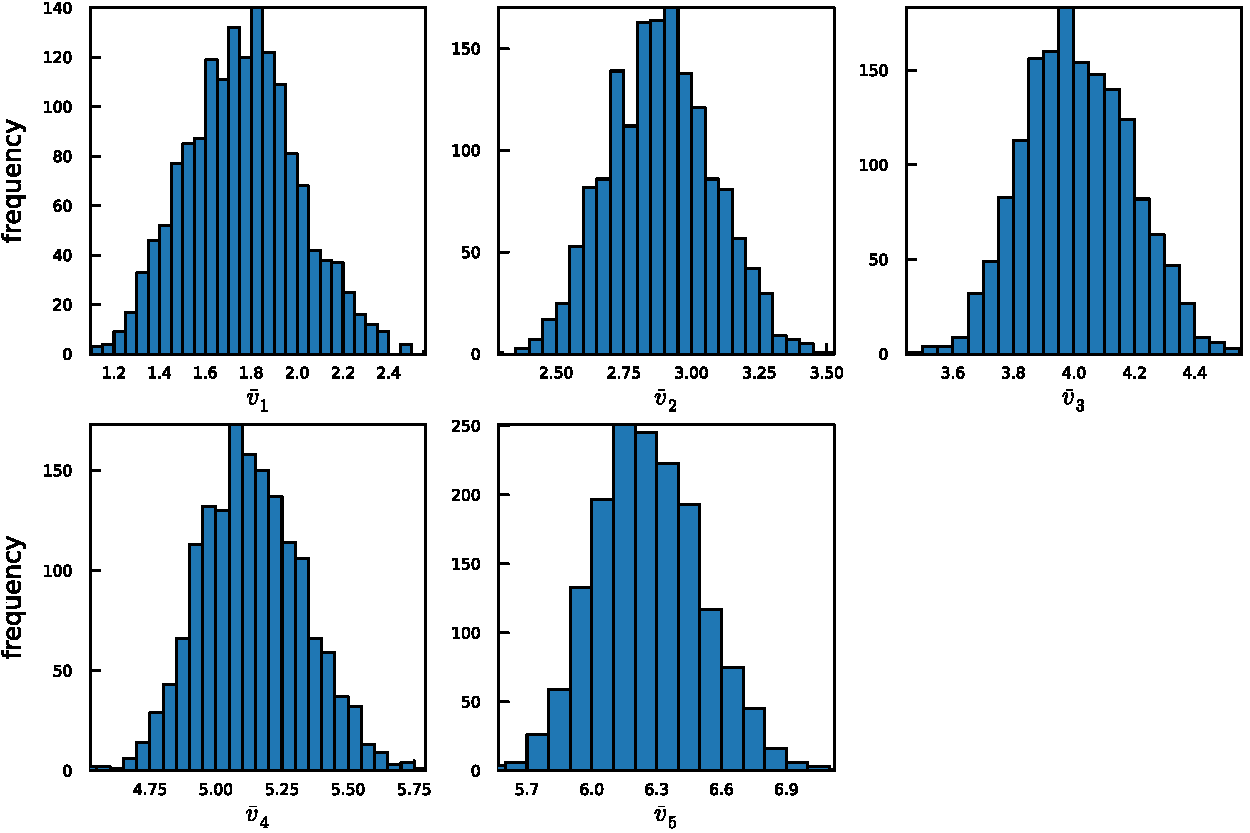
\includegraphics[width=\linewidth]{sample means N=1000}
        \subcaption{Histogram of the sample means for \(N = 1000\).}
        \label{fig:hist_mean:a}
    \end{minipage}
    \hfill
    \begin{minipage}[t]{0.8\linewidth}
        \centering
        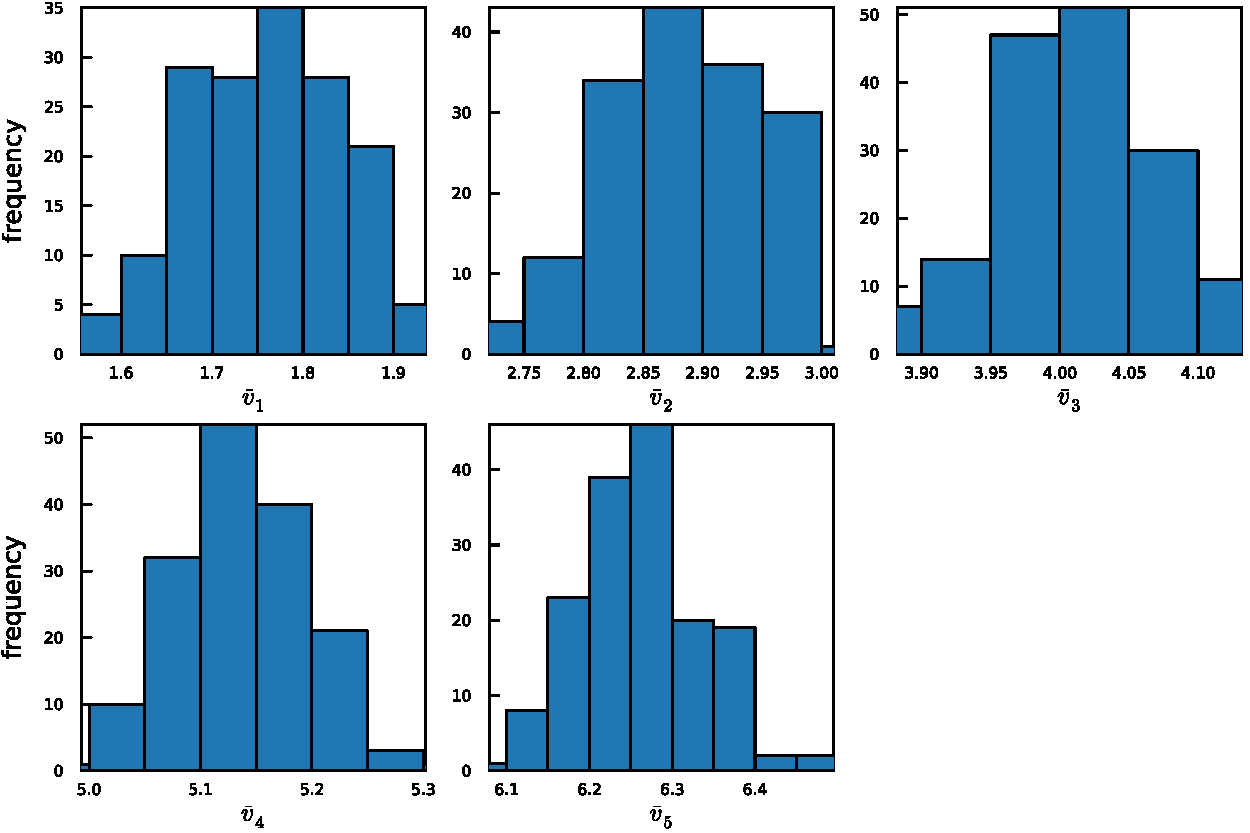
\includegraphics[width=\linewidth]{sample means N=10000}
        \subcaption{Histogram of the sample means for \(N = 10000\).}
        \label{fig:hist_mean:b}
    \end{minipage}
    \caption{Take \(N = 1000\) and \(N = 10000\) as each sample size
        for \(v_1\), \(v_2\), \(\ldots\), \(v_5\) from all \(M\) values
        and histogram their mean values.}
    \label{fig:hist_mean}
\end{figure}

The true variance of the means is defined as
%
\begin{equation}\label{eq:varva}
    \hat{\mathbb{V}}(v_a) = \frac{ 1 }{ M/N - 1 }
    \sum_{\eta=1}^{M/N} (\bar{v}_{a,\eta} - \barhat{v}_a)^2.
\end{equation}
%
And the true standard deviation of the means is defined as
%
\begin{equation}
    \sgbar{a} = \sqrt{\hat{\mathbb{V}}(v_a)}.
\end{equation}
%
Therefore, we have list the true standard deviation of the means
\(\sgbar{a}\) for \(a = 1\), \(\ldots\), \(5\) and \(N = 1000\) and \(10000\)
in Table~\ref{tab:truestd}.
We can see that the \(\sgbar{a}\)'s for \(N = 10000\) are much smaller than
when \(N = 1000\). This is consistent with the results in Figure~\ref{fig:hist_mean}
since the distribution of \(\bar{v}_a\) is narrower when \(N = 10000\) since
we are averaging more values in one sample.

\begin{table}[H]
    \centering
    \caption{The true standard deviation of the means
        \(\sgbar{a}\) for \(a = 1\), \(\ldots\), \(5\) and \(N = 1000\) and \(10000\).}
    \label{tab:truestd}
    \begin{tabular}{@{}cccccc@{}}
        \toprule
        \(N\)     & \(\sgbar{1}\) & \(\sgbar{2}\) & \(\sgbar{3}\) & \(\sgbar{4}\) & \(\sgbar{5}\) \\
        \midrule
        \(1000\)  & \(0.24312\)   & \(0.19294\)   & \(0.17706\)   & \(0.19428\)   & \(0.24565\)   \\
        \(10000\) & \(0.08173\)   & \(0.06387\)   & \(0.05607\)   & \(0.05901\)   & \(0.07425\)   \\
        \bottomrule
    \end{tabular}
\end{table}


\Question{} You can now determine the true autocorrelation function for each variable,
\(\hat{C}_{v_a}(n)\), which is given by
%
\begin{equation}
    \hat{C}_{v_a}(n) = \frac{ 1 }{ M - n }
    \sum_{i=1}^{M-n} (v_{a,i} - \barhat{v}_a) (v_{a,i + n} - \barhat{v}_a).
\end{equation}
%
Here \(n\) goes from \(0\) to some maximum value \(n_\textnormal{cut}\) with
\(n_\textnormal{cut} \ll M\).
Plot \(\hat{C}_{v_a}(n) / \hat{C}_{v_a}(0)\) versus \(n\) for \(a = 1\), \(\ldots\), \(5\).

\Answer{}
The code snippet for the true autocorrelation function is shown in Snippet~\ref{lst:truecor}.
We can see that the true autocorrelation function is different from the sample's
autocorrelation functions~\eqref{eq:sampleautocor}.

\begin{algorithm}
    \caption{The true autocorrelation function \(\hat{C}_{v_a}(n)\) for variable \(v_a\).}
    \label{lst:truecor}
    \begin{juliacode}
        function truecor(population::Population, n)
            μ = mean(population)
            return sum(firstindex(population):(lastindex(population) - n)) do i
                (population[i] - μ) * (population[i + n] - μ)
            end / (length(population) - n)
        end
    \end{juliacode}
\end{algorithm}

We plot \(\hat{C}_{v_a}(n) / \hat{C}_{v_a}(0)\) as a function of \(n\) for \(a = 1\), \(\ldots\),
\(5\) in Figure~\ref{fig:truecor}.
Here the \(n_\textnormal{cut}\) is \(300\) since it is large enough to see the trend
that
%
\begin{equation}
    \lim_{n \rightarrow \infty} \frac{ \hat{C}_{v_a}(n) }{ \hat{C}_{v_a}(0) } = 0.
\end{equation}

\begin{figure}[h]
    \centering
    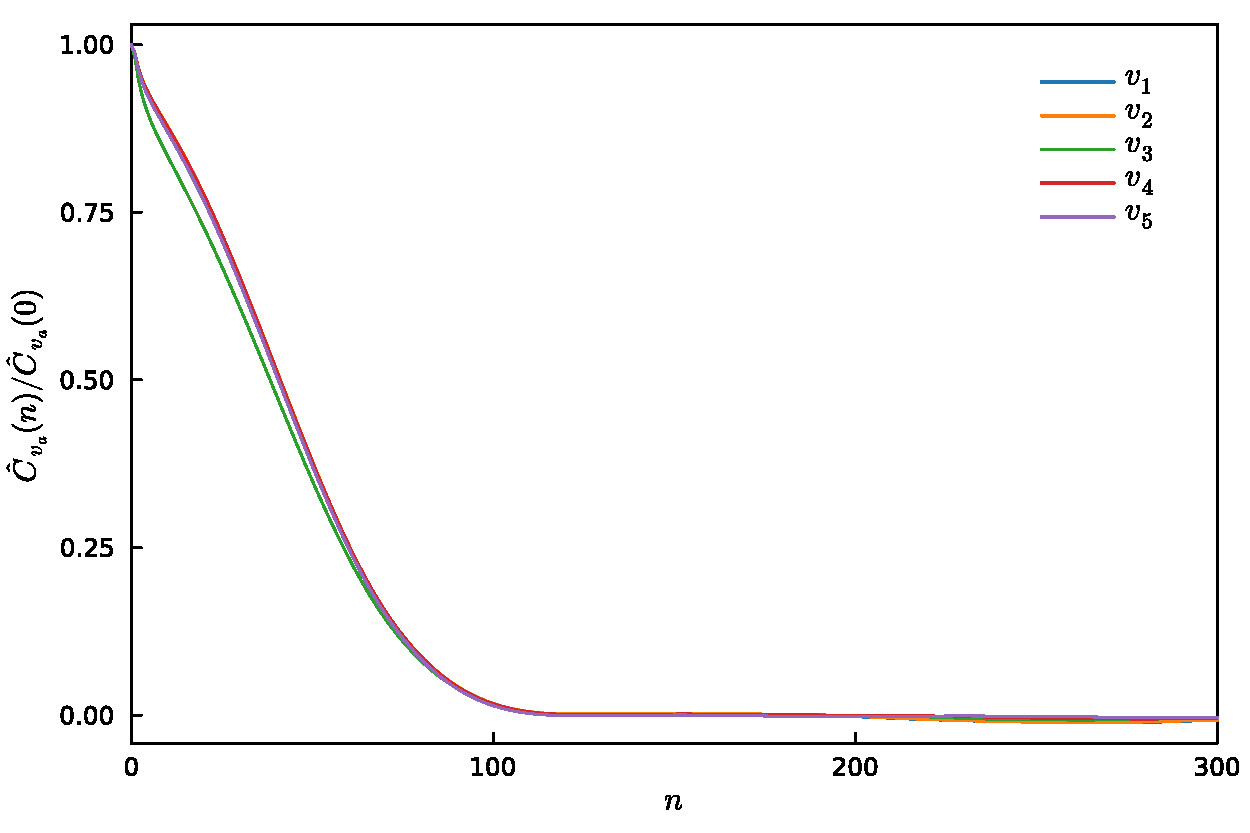
\includegraphics[width=0.8\textwidth]{Cn_C0}
    \caption{\(\hat{C}_{v_a}(n) / \hat{C}_{v_a}(0)\) as a function of \(n\) for
        \(a = 1\), \(\ldots\), \(5\).}
    \label{fig:truecor}
\end{figure}

One thing to notice that these ratios \(\hat{C}_{v_a}(n) / \hat{C}_{v_a}(0)\)
is just close to \(0\), not exactly at \(0\). And they are not monotonically decreasing
to \(0\), but still have some wiggles until very large \(N\), as shown in
Figure~\ref{fig:truecorlarge}.

\begin{figure}[h]
    \centering
    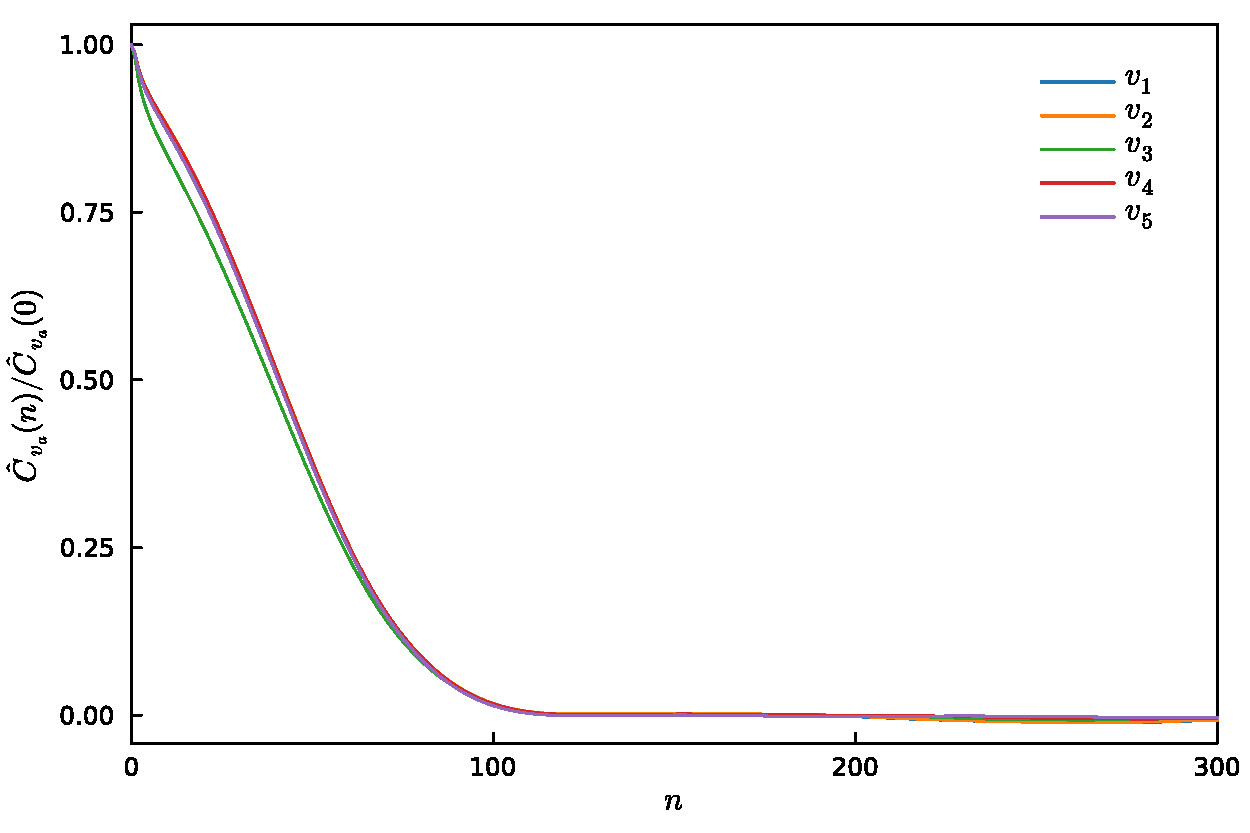
\includegraphics[width=0.8\textwidth]{Cn_C0}
    \caption{\(\hat{C}_{v_a}(n) / \hat{C}_{v_a}(0)\) as a function of \(n\)
        for \(n\) in range \(200 - 2000\).}
    \label{fig:truecorlarge}
\end{figure}


\Question{} Find the integrated autocorrelation time
%
\begin{equation}\label{eq:tau}
    \hat{\tau}_{v_a} \equiv \frac{ 1 }{ 2 \hat{C}_{v_a}(0) }
    \sum_{n=-n_\textnormal{cut}}^{n=n_\textnormal{cut}} \hat{C}_{v_a}(n).
\end{equation}
%
Estimate a value for \(n_\textnormal{cut}\) from your plots.
\(n_\textnormal{cut}\) should be large enough that \(\hat{C}_{v_a}(n) / \hat{C}_{v_a}(0)\)
has gotten close enough to zero that the value of \(\hat{\tau}_{v_a}\)
is not affected by modest changes in \(n_\textnormal{cut}\).

\Answer{}
Equation \eqref{eq:tau} can be rewritten as
%
\begin{equation}
    \hat{\tau}_{v_a} = \frac{ 1 }{ 2 \hat{C}_{v_a}(0) }
    \biggl( 2\sum_{n=1}^{n_\textnormal{cut}} \hat{C}_{v_a}(n) + \hat{C}_{v_a}(0) \biggr)
    = \frac{ \sum_{n=1}^{n_\textnormal{cut}} \hat{C}_{v_a}(n) }{ \hat{C}_{v_a}(0) }
    + \frac{ 1 }{ 2 }
\end{equation}
%
since the autocorrelation function is symmetric.
Therefore, we select \(n_\textnormal{cut} = 200\) since it is enough for \(\hat{\tau}_{v_a}\)
to converge.
The final results are shown in Figure~\ref{fig:tau} and Table~\ref{tab:tau}.

\begin{figure}[h]
    \centering
    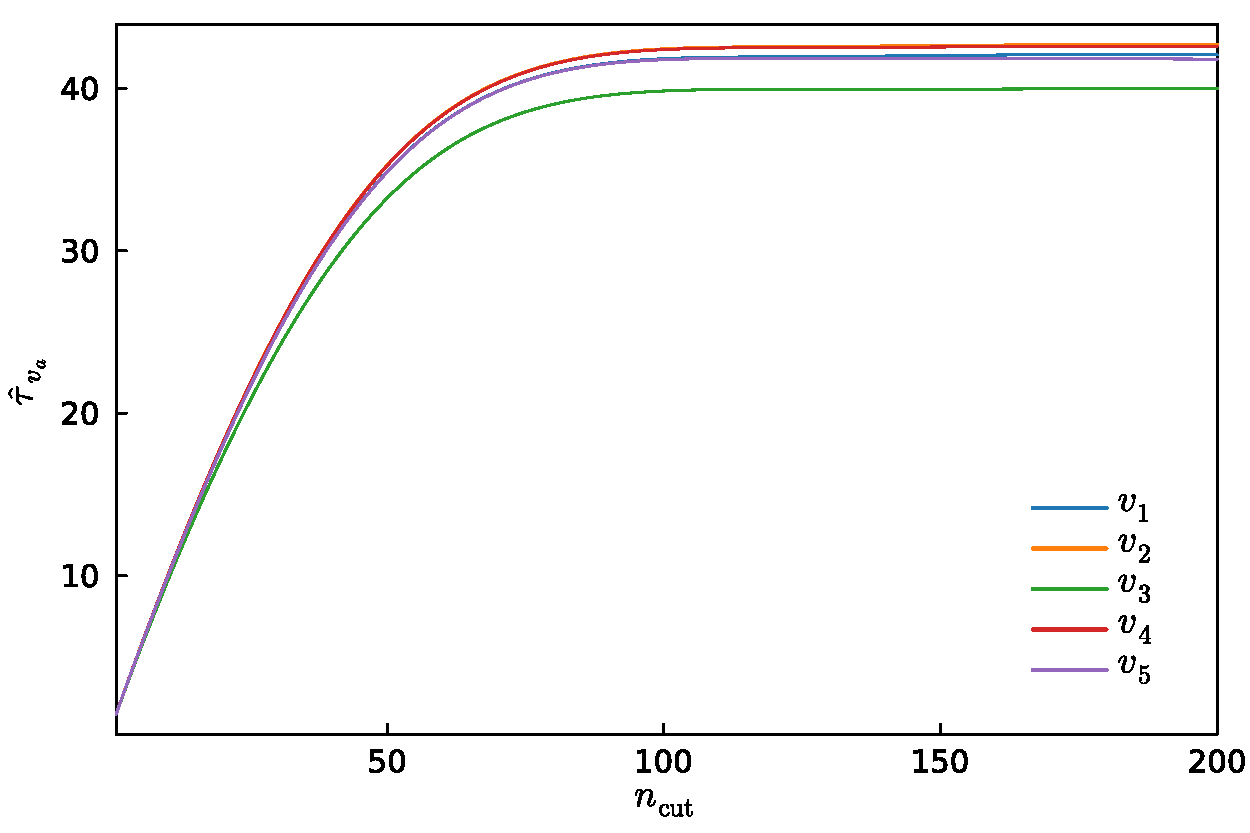
\includegraphics[width=0.8\textwidth]{tau}
    \caption{The integrated autocorrelation time \(\hat{\tau}_{v_a}\) as a
        function of \(n_\textnormal{cut}\) for \(a = 1\), \(\ldots\), \(5\).}
    \label{fig:tau}
\end{figure}

\begin{table}
    \centering
    \caption{The integrated autocorrelation time \(\hat{\tau}_{v_a}\) with
        \(n_\textnormal{cut} = 200\) for \(a = 1\), \(\ldots\), \(5\).}
    \label{tab:tau}
    \begin{tabular}{@{}ccccc@{}}
        \toprule
        \(\hat{\tau}_{v_1}\) & \(\hat{\tau}_{v_2}\) & \(\hat{\tau}_{v_3}\) & \(\hat{\tau}_{v_4}\) & \(\hat{\tau}_{v_5}\) \\
        \midrule
        \(42.08254\)         & \(42.70645\)         & \(40.00157\)         & \(42.60346\)         & \(41.80298\)         \\
        \bottomrule
    \end{tabular}
\end{table}


\Question{} Calculate the true standard deviation of the data, i.e.,
%
\begin{equation}\label{eq:truestd}
    \hat{\sigma}_{v_a} \equiv \sqrt{\frac{ 1 }{ M - 1 }
        \sum_{i=1}^M \bigl( v_{a,i} - \barhat{v}_a \bigr)^2}.
\end{equation}
%
For a sample of size \(N\), we should have
%
\begin{equation}\label{eq:relation}
    \sgbar{a} = \sqrt{\frac{ 2 \hat{\tau}_{v_a} }{ N }} \hat{\sigma}_{v_a}.
\end{equation}
%
Does this relation hold for your analysis?

\Answer{}
In Equation~\eqref{eq:truestd}, we are treating all \(M\) values as a sample,
not the population.
That is why we divide it by \(M - 1\), not \(M\).

The true standard deviations of all \(M\) data for each variable are
listed in Table~\ref{tab:std}.
While the true standard deviation of the means
\(\sgbar{a}\) for \(a = 1\), \(\ldots\), \(5\) and \(N = 1000\) and \(10000\) are
listed in Table~\ref{tab:truestd}.

\begin{table}[H]
    \centering
    \caption{The true standard deviations of all \(M\) data for each variable.}
    \label{tab:std}
    \begin{tabular}{@{}ccccc@{}}
        \toprule
        \(\hat{\sigma}_{v_1}\) & \(\hat{\sigma}_{v_2}\) & \(\hat{\sigma}_{v_3}\) & \(\hat{\sigma}_{v_4}\) & \(\hat{\sigma}_{v_5}\) \\
        \midrule
        \(0.751404\)           & \(0.461788\)           & \(0.406673\)           & \(0.457226\)           & \(0.742713\)           \\
        \bottomrule
    \end{tabular}
\end{table}

In the following text, we define
%
\begin{equation}
    \hat{s}_{\bar{v}_a,N} \equiv \sqrt{\frac{ 2 \hat{\tau}_{v_a} }{ N }} \hat{\sigma}_{v_a}
\end{equation}
%
and compare them with \(\sgbar{a}\) to see if they match.

All the values of \(\sgbar{a}\), \(\hat{s}_{\bar{v}_a,N}\) and their differences
for each variable for each \(N\) are listed in Table~\ref{tab:s}.
We can see their expected values (\(\sgbar{a}\)) and our evaluated values
(\(\hat{s}_{\bar{v}_a,N}\)) are different by some small amounts.
It means that relation~\eqref{eq:relation} holds for our analysis.

\begin{table}[H]
    \centering
    \caption{Compare \(\sgbar{a}\) and \(\hat{s}_{\bar{v}_a,N}\) for
    \(a = 1\), \(\ldots\), \(5\) and \(N = 1000\) and \(10000\).}
    \label{tab:s}
    \begin{tabular}{@{}ccccc@{}}
        \toprule
        \(N\)     & variable                 & \(\sgbar{a}\) & \(\hat{s}_{\bar{v}_a,N}\) & \(\sgbar{a}-\hat{s}_{\bar{v}_a,N}\) \\
        \midrule
        \(1000\)  & \multirow{2}{*}{\(v_1\)} & \(0.24312\)   & \(0.25148\)               & \num{-8.36E-03}                     \\
        \(10000\) &                          & \(0.08173\)   & \(0.07952\)               & \num{2.20E-03}                      \\
        \cmidrule{1-2}
        \(1000\)  & \multirow{2}{*}{\(v_2\)} & \(0.19294\)   & \(0.1986\)                & \num{-5.66E-03}                     \\
        \(10000\) &                          & \(0.06387\)   & \(0.0628\)                & \num{1.06E-03}                      \\
        \cmidrule{1-2}
        \(1000\)  & \multirow{2}{*}{\(v_3\)} & \(0.17706\)   & \(0.18037\)               & \num{-3.32E-03}                     \\
        \(10000\) &                          & \(0.05607\)   & \(0.05704\)               & \num{-9.73E-04}                     \\
        \cmidrule{1-2}
        \(1000\)  & \multirow{2}{*}{\(v_4\)} & \(0.19428\)   & \(0.19738\)               & \num{-3.10E-03}                     \\
        \(10000\) &                          & \(0.05901\)   & \(0.06242\)               & \num{-3.41E-03}                     \\
        \cmidrule{1-2}
        \(1000\)  & \multirow{2}{*}{\(v_5\)} & \(0.24565\)   & \(0.24919\)               & \num{-3.54E-03}                     \\
        \(10000\) &                          & \(0.07425\)   & \(0.0788\)                & \num{-4.56E-03}                     \\
        \bottomrule
    \end{tabular}
\end{table}


\Question{} Calculate the true covariance matrix for the data, defined by
%
\begin{equation}
    \hat{c}_{v_a, v_b} = \frac{ 1 }{ M }
    \sum_{i=1}^M (v_{a,i} - \barhat{v}_a) (v_{b,i} - \barhat{v}_b).
\end{equation}
%
It is customary to define a normalized version of \(\hat{c}_{v_a, v_b}\) by
%
\begin{equation}
    \hat{\rho}_{v_a, v_b} \equiv \frac{ \hat{c}_{v_a, v_b} }{ \hat{\sigma}_{v_a} \hat{\sigma}_{v_b} }.
\end{equation}
%
Since \(\hat{c}_{v_a, v_b} = \hat{\sigma}_{v_a}^2\),
\(\hat{\rho}_{v_a, v_b}\) has ones on the diagonals and the off diagonals give a
ready measure of the covariance between variables.

\Answer{}
The covariance matrix is
%
\begin{equation}
    \hat{c}_{v_a, v_b} =
    \begin{bmatrix}
        0.7514  & 0.54797 & 0.34454 & 0.17229 & 0.00005 \\
        0.54797 & 0.46179 & 0.3756  & 0.27276 & 0.16991 \\
        0.34454 & 0.3756  & 0.40667 & 0.37322 & 0.33976 \\
        0.17229 & 0.27276 & 0.37322 & 0.45723 & 0.54124 \\
        0.00005 & 0.16991 & 0.33976 & 0.54124 & 0.74271
    \end{bmatrix}.
\end{equation}
%
And the normalized version of the covariance, i.e., the
\emph{(Pearson) correlation coefficient}, is
%
\begin{equation}
    \hat{\rho}_{v_a, v_b} =
    \begin{bmatrix}
        1       & 0.93025 & 0.62327 & 0.29395 & 0.00007 \\
        0.93025 & 1       & 0.86674 & 0.59359 & 0.29012 \\
        0.62327 & 0.86674 & 1       & 0.86551 & 0.61821 \\
        0.29395 & 0.59359 & 0.86551 & 1       & 0.92878 \\
        0.00007 & 0.29012 & 0.61821 & 0.92878 & 1
    \end{bmatrix}.
\end{equation}
%
We can see the diagonals of the correlation coefficient matrix are indeed \(1\).


\Question{} Now, pick two groups of data from the full universe of data. One should have
\(N = 1000\) and the other should have \(N = 10000\). These two groups represent results one
might get from simulations. We want to see how well these groups reproduced the true
statistical results for these data.
Estimate the autocorrelation function \(C_{v_a}(n)\) from these two groups and the integrated
autocorrelation time. Use these to determine the standard deviation of the mean
\(\sigma_{\bar{v}_a,N}\). Compare this with the results from the universe of data. Also
compare the normalized covariance matrix \(\hat{\rho}_{v_a, v_b}\) from these small samples
with the universe of data.

\Answer{}
The sample's autocorrelation function is
%
\begin{equation}\label{eq:sampleautocor}
    C_{v_a}(n) = \frac{ 1 }{ N - n - 1 }
    \sum_{i=1}^{N-n} (v_{a,i} - \bar{v}_a) (v_{a,i + n} - \bar{v}_a).
\end{equation}
%
And the sample's integrated autocorrelation time is defined as
%
\begin{equation}\label{eq:sampletau}
    \tau_{v_a} = \frac{ 1 }{ 2 C_{v_a}(0) }
    \sum_{n=-n_\textnormal{cut}}^{n=n_\textnormal{cut}} C_{v_a}(n).
\end{equation}
%
In addition, the standard deviation of the mean satisfy the relation
%
\begin{equation}
    \sigma_{\bar{v}_a,N} = \sqrt{\frac{ 2\tau_{v_a} }{ N }} \sigma_{v_a},
\end{equation}
%
just as what we saw in~\eqref{eq:relation}, where the standard deviation of the sample is
%
\begin{equation}
    \sigma_{v_a} = \sqrt{\frac{ 1 }{ N - 1 } \sum_{i=1}^N (v_{a,i} - \bar{v}_a)^2}.
\end{equation}
